\documentclass[11pt,a4paper]{article}
\usepackage[T1]{fontenc}
\usepackage{newtxtext,newtxmath}
\usepackage[margin=22mm]{geometry}
\usepackage{amsmath,bm,booktabs,longtable,tabularx,graphicx,enumitem,float}
\usepackage{xurl}
\usepackage[hidelinks]{hyperref}
\usepackage{cite}
\graphicspath{{figures/}}
\numberwithin{equation}{section}
\renewcommand{\thesection}{S\arabic{section}}
\renewcommand{\thefigure}{S\arabic{figure}}
\renewcommand{\thetable}{S\arabic{table}}
\setlength{\emergencystretch}{2em}
\setlist{nosep}
\allowdisplaybreaks
\newcommand{\R}{\mathsf R}
\newcommand{\J}{\mathsf J}
\newcommand{\ii}{\mathrm i}
\begin{document}
\title{Supplementary Material\\[5pt]\large Task-Oriented Modeling of AI Data Center Plants for Resonance Analysis}
\author{Ruizhi Yu, Wei Gu, Shuai Lu, Suhan Zhang and Shiqi Fu}
\date{23 September 2026}
\maketitle
This document gives the supply-block equations, electrical parameters, workload construction, single-block equivalent and additional comparison results of the accompanying paper.
The electrical equations follow Zhao and Zhao \cite{zhao2026dynamic}.
Task timing follows Ko and Zhu \cite{ko2026oscillations}, with power levels from the National Laboratory of the Rockies (NLR) workload dataset \cite{vercellino2026measurement}.
The new material concerns their plant-level composition and its comparison with the single-block equivalent.
All numerical results in this document come from saved project results.
No additional simulations are introduced by this document.
\tableofcontents
\clearpage
\section{Electrical Model and Power Accounting}
\label{sec:electrical}
\subsection{Conventions and state variables}
A reproducible plant model requires consistent device bases and connection signs.
Each supply block consists of a unit transformer, an active front end (AFE), a voltage source inverter (VSI), a power supply unit (PSU) array and a server DC--DC stage.
The unit transformer belongs to the algebraic network, and the four converter stages carry the differential states of the block.
Each supply block uses its own three-phase rating $S_n$ as the power base.
The network uses $S_b=200$~MVA and $\omega_b=2\pi60$~rad/s.
Time is in seconds.
Per-unit inductances and capacitances multiply derivatives divided by $\omega_b$.
Controller integrators retain the unscaled time derivatives used in the source equations.
The reference speed is $\omega_s=1$.

The local AFE frame rotates by the phase-locked loop (PLL) angle $\theta$.
Define
\begin{equation}
\R(\theta)=\begin{bmatrix}\cos\theta&\sin\theta\\-\sin\theta&\cos\theta\end{bmatrix},\qquad
\J=\begin{bmatrix}0&-1\\1&0\end{bmatrix}.
\end{equation}
Here $\bm v_g$ is the voltage at the low-voltage terminal of the unit transformer in network coordinates.
The rectifier current $\bm i_a$ is positive into the supply block.
The VSI uses a separate synchronous frame with voltage $\bm v_v$ and converter current $\bm i_c$.

One supply block has 21 differential states.
The AFE contributes $\theta$, $\epsilon$, $\bar v_q$, the two entries of $\bm i_a$, $\xi_a$ and the two entries of $\bm\gamma_a$.
The VSI contributes the two entries of each of $\bm i_c$, $\bm v_v$, $\bm\xi_v$ and $\bm\gamma_v$.
The remaining states are the shared DC-link voltage $v_d$, the PSU output voltage $v_p$ and integrator $\xi_p$, and the server voltage $v_e$ and integrator $\xi_e$.
The following vector equations count each two-entry vector as two states.
The accompanying paper writes $v_{\rm dc}$, $v_{\rm psu}$ and $v_{\rm s}$ for $v_d$, $v_p$ and $v_e$.

\subsection{AFE rectifier}
The rectifier synchronizes to the unit-transformer voltage and regulates the shared DC link.
Let $\bm v_a=\R(\theta)\bm v_g$.
Its equations are
\begin{align}
\dot\theta&=\omega_b(\omega_{\rm pll}-\omega_s), & \dot\epsilon&=\bar v_q,\\
\dot{\bar v}_q&=\omega_{\rm lp}(v_{a,q}-\bar v_q), &
\omega_{\rm pll}&=\omega_s+k_{p,\rm pll}\bar v_q+k_{i,\rm pll}\epsilon,\\
\frac{\ell_a}{\omega_b}\dot{\bm i}_a&=\bm v_a-v_d\bm m_a-r_a\bm i_a+\omega_{\rm pll}\ell_a\J\bm i_a,\\
\dot\xi_a&=v_d^\star-v_d, & \dot{\bm\gamma}_a&=\bm i_a-\bm i_a^\star,\\
\bm i_a^\star&=\begin{bmatrix}k_{p,da}(v_d^\star-v_d)+k_{i,da}\xi_a\\0\end{bmatrix},\\
\bm m_a&=\frac{k_{p,ca}(\bm i_a-\bm i_a^\star)+k_{i,ca}\bm\gamma_a+\omega_{\rm pll}\ell_a\J\bm i_a}{v_d}.
\end{align}
A superscript $\star$ denotes a reference value.
The constants $r_a$ and $\ell_a$ are the AFE filter resistance and inductance.
Subscripts $da$ and $ca$ identify the DC-voltage and current controllers.
The current-controller error and the coupling signs follow the source model \cite{zhao2026dynamic}.
Another rectifier convention would change the model.

\subsection{VSI and shared DC link}
The VSI regulates its output voltage while drawing energy from the rectifier DC link.
With reference $\bm v_v^\star=[v_u^\star,0]^{\mathsf T}$, its equations are
\begin{align}
\frac{\ell_v}{\omega_b}\dot{\bm i}_c&=v_d\bm m_v-\bm v_v-r_v\bm i_c+\omega_s\ell_v\J\bm i_c,\label{eq:vsi-current}\\
\frac{c_v}{\omega_b}\dot{\bm v}_v&=\bm i_c-\bm i_o+\omega_s c_v\J\bm v_v,\\
\dot{\bm\xi}_v&=\bm v_v^\star-\bm v_v, & \dot{\bm\gamma}_v&=\bm i_c^\star-\bm i_c,\\
\bm i_c^\star&=k_{p,vv}(\bm v_v^\star-\bm v_v)+k_{i,vv}\bm\xi_v-\omega_s c_v\J\bm v_v,\\
\bm m_v&=\frac{k_{p,cv}(\bm i_c^\star-\bm i_c)+k_{i,cv}\bm\gamma_v-\omega_s\ell_v\J\bm i_c}{v_d},\label{eq:vsi-modulation}\\
\frac{c_d}{\omega_b}\dot v_d&=\bm m_a^{\mathsf T}\bm i_a-\bm m_v^{\mathsf T}\bm i_c.
\end{align}
Here $r_v$, $\ell_v$ and $c_v$ are the VSI filter parameters, $c_d$ is the DC-link capacitance, and $\bm i_o$ is the current drawn by the PSU array.
Subscripts $vv$ and $cv$ denote its voltage and current controllers.
The DC-link equation couples both converters through their current balance.
The study represents online double-conversion operation.

\subsection{PSU array and server DC--DC stage}
The positive-sequence PSU equivalent converts its AC input into a common DC supply.
Let $g_p$ be its controlled input conductance and $i_p$ its DC output current.
Then
\begin{align}
\frac{c_p}{\omega_b}\dot v_p&=\frac{(g_p-r_p g_p^2)\bm v_v^{\mathsf T}\bm v_v}{3v_p}-i_p, &
\dot\xi_p&=v_p^\star-v_p,\\
g_p&=k_{p,vp}(v_p^\star-v_p)+k_{i,vp}\xi_p, & \bm i_o&=g_p\bm v_v.
\end{align}
The parameters $r_p$ and $c_p$ represent the PSU equivalent resistance and capacitance.
The downstream DC--DC stage has a fast current loop represented by its commanded current $i_e$, with
\begin{align}
\frac{c_e}{\omega_b}\dot v_e&=i_e-g_e v_e, & \dot\xi_e&=v_e^\star-v_e,\\
g_e&=\frac{p_{\rm load}}{3(v_e^\star)^2}, &
i_e&=k_{p,ve}(v_e^\star-v_e)+k_{i,ve}\xi_e, &
i_p&=\frac{v_e}{v_p}i_e.
\end{align}
The factor 3 follows the source model's three-phase power convention.
The input $p_{\rm load}$ is the prescribed server power on the block base at $v_e=v_e^\star$.
The instantaneous power of the modeled load is $3g_e v_e^2$, so it equals $p_{\rm load}$ at the voltage reference.
This distinction matters when interpreting internal voltage excursions.
The server power of the hall sets this command.
It is not an additional current injection at the PCC.

\subsection{Hall and network connections}
Each hall has one common feeder and four parallel supply blocks.
Each block has its own 3~MVA unit transformer and converters.
The four blocks of hall $h$ have identical parameters, and each receives the command $p_{\rm load}=P_{{\rm IT},h}/(4S_n)$, where $P_{{\rm IT},h}$ is the server power of the hall defined in Section~\ref{sec:allocation}.
The AC input power of a block is the active power that it draws at the low-voltage terminal of its unit transformer, and $P_{{\rm AC},h}$ denotes its sum over the four blocks of hall $h$.
The cooling load connects to the hall bus after the common feeder and before the unit transformers.
Auxiliary loads connect to the two medium-voltage buses.
The full model keeps both medium-voltage buses, both main transformers, the 12 feeders and the 48 unit transformers as separate elements.
Section~\ref{sec:equivalent} describes how the single-block equivalent merges them.

The current drawn from the network by supply block $n$ is
\begin{equation}
\bm i_{n,\rm sys}=\frac{S_n}{S_b}\R(\theta_n)^{\mathsf T}\bm i_{a,n}.
\end{equation}
With the network voltage phasors $V$, generator injections $I_G$ and explicit load withdrawals $I_L$, nodal balance is $YV=I_G-I_L$.
A load represented as an admittance is included in $Y$ and is excluded from $I_L$.
The network is algebraic and retains the line and transformer impedances and the feeder charging.

In the full model, the cooling power of a hall at the operating point is 17\% of the AC input power of its supply blocks.
The total auxiliary power is 3\% of the AC input power of all supply blocks, divided equally between the medium-voltage sections.
Cooling uses a constant-power representation and the auxiliaries use constant impedance.
With the AC input power $P_{n,\rm AC}$ of block $n$ at the operating point, the static demand at bus~8 is
\begin{equation}
P_{8,\rm residual}=100-1.20\sum_n P_{n,\rm AC}\quad\mathrm{MW}.
\end{equation}
The original 35~Mvar remains as a static impedance load.
Collector losses are accounted for by the network.
The PCC power is the sum of the powers entering the main transformers, so it includes these losses.
The single-block equivalent keeps the static loads of the full model.
They are not adjusted to cancel the loss error of the equivalent.

The external system has a fourth-order synchronous machine with excitation and turbine-governor dynamics at bus~1, a droop grid-forming converter at bus~2 and a phase-locked-loop grid-following converter at bus~3.
Their equations and parameter conventions follow the modified nine-bus reference in the supplement of \cite{zhao2026dynamic}.
The implementation uses the source-current feed-forward sign $-1$ and the q-axis voltage convention for the grid-following converter.
The accompanying data files give all grid parameter values and network branches.
These grid devices contribute 37 states, so a model with $N$ supply blocks has $37+21N$ states.
The full model has $N=48$ blocks and 1045 states, and the single-block equivalent has $N=1$ and 58 states.

\section{Electrical Parameters and Workload Inputs}
\subsection{Device design}
Independent parameter draws describe differences between halls while preserving identical chains inside each hall.
A PCG64 generator uses seed 20260919.
The draw order is section, hall, the nine passive elements, seven controller bandwidths, the PLL filter frequency, feeder length and unit-transformer impedance.
The numerical ranges are study assumptions, rather than a measured distribution of data-center equipment.

\begin{table}[H]
\centering
\caption{Nominal Device Parameters and Uniform Draw Ranges}
\begin{tabular}{llll}
\toprule
Quantity & Symbol & Nominal & Draw range\\\midrule
AFE resistance & $r_a$ & 0.003 & 0.0027 to 0.0033\\
AFE inductance & $\ell_a$ & 0.05 & 0.045 to 0.055\\
DC-link capacitance & $c_d$ & 2.0 & 1.8 to 2.2\\
VSI resistance & $r_v$ & 0.003 & 0.0027 to 0.0033\\
VSI inductance & $\ell_v$ & 0.05 & 0.045 to 0.055\\
VSI capacitance & $c_v$ & 0.2 & 0.18 to 0.22\\
PSU resistance & $r_p$ & 0.005 & 0.0045 to 0.0055\\
PSU capacitance & $c_p$ & 2.0 & 1.8 to 2.2\\
Server-side capacitance & $c_e$ & 0.2 & 0.18 to 0.22\\\bottomrule
\end{tabular}
\end{table}
All entries are per unit on the chain base.
The voltage references are $v_d^\star=v_u^\star=v_p^\star=1$ and $v_e^\star=0.5$.
Nominal values originate from \cite{zhao2026dynamic}.
The VSI voltage-loop bandwidth is 80~Hz in this study, whereas the source Table I uses 100~Hz.

\begin{table}[H]
\centering
\caption{Controller Bandwidths and Tuning Damping Ratios}
\begin{tabular}{lrrr}
\toprule
Loop & Nominal in Hz & Range in Hz & $\zeta$\\\midrule
PLL & 20 & 16 to 24 & 0.707\\
AFE DC voltage & 5 & 4 to 6 & 1\\
AFE current & 200 & 160 to 240 & 0.707\\
VSI voltage & 80 & 64 to 96 & 1\\
VSI current & 400 & 320 to 480 & 1\\
PSU voltage & 10 & 8 to 12 & 1\\
Server voltage & 100 & 80 to 120 & 1\\\bottomrule
\end{tabular}
\end{table}
The PLL low-pass frequency is uniform from 80 to 120~Hz.
Gains follow the bandwidth rule in \cite{zhao2026dynamic}.
With $\omega_n=2\pi f_{\rm bw}$, the voltage loop has $k_p=2\zeta\omega_n C/\omega_b$ and $k_i=\omega_n^2 C/\omega_b$.
The current loop has $k_p=2\zeta\omega_n L/\omega_b-R$ and $k_i=\omega_n^2 L/\omega_b$.
The PLL uses $k_p=2\zeta\omega_n/\omega_b$ and $k_i=\omega_n^2/\omega_b$.
Gains are derived from each draw and are not independent random parameters.

Exact values for all 12 halls, including every derived gain, are in \path{data/design.json}.
Table~\ref{tab:hall-design} gives the controller and connection parameters that identify the hall differences.
The data file retains full precision.
\begin{table}[H]
\centering\small
\caption{Hall Design Summary. Frequencies in Hz, Feeder Length in km, Transformer Impedance in Percent.}
\label{tab:hall-design}
\begin{tabular}{rrrrrrr}\toprule
Hall & PLL & AFE voltage & VSI voltage & PSU voltage & Feeder & Transformer\\\midrule
1 & 19.17 & 4.22 & 77.58 & 8.14 & 0.92 & 5.93 \\
2 & 18.67 & 5.39 & 91.66 & 10.52 & 0.95 & 5.74 \\
3 & 18.25 & 5.47 & 71.17 & 10.50 & 0.65 & 5.26 \\
4 & 23.56 & 5.52 & 72.54 & 10.90 & 1.25 & 5.30 \\
5 & 17.39 & 5.88 & 73.97 & 9.48 & 1.49 & 5.77 \\
6 & 17.92 & 5.54 & 71.70 & 10.34 & 1.23 & 5.01 \\
7 & 17.93 & 4.85 & 64.84 & 8.17 & 1.01 & 5.21 \\
8 & 22.56 & 4.30 & 94.19 & 10.87 & 1.28 & 5.42 \\
9 & 20.33 & 5.97 & 86.54 & 9.54 & 0.22 & 5.54 \\
10 & 23.18 & 5.88 & 94.08 & 9.07 & 0.83 & 5.37 \\
11 & 19.71 & 4.45 & 95.56 & 10.59 & 0.94 & 5.12 \\
12 & 21.27 & 5.23 & 73.92 & 10.07 & 0.94 & 5.54 \\
\bottomrule\end{tabular}\end{table}


\subsection{Network data}
The main transformers are each 100~MVA with 8.5\% impedance and assumed $X/R=35$.
Unit transformers are 3~MVA with a uniformly drawn impedance of 5\% to 6\% and assumed $X/R=6$.
Their ratings are compatible with the repeated power-block representation discussed in \cite{ross2025emt}; the complete topology is a study configuration.

Each 34.5~kV feeder has a drawn length from 0.2 to 1.5~km.
Its series impedance is $0.046+\ii0.043$~$\Omega$ per 1000~ft, with capacitive reactance coefficient $0.042$~M$\Omega\cdot1000$~ft.
These values come from Southwire SPEC 80214, revision 1.000.021, for a 35~kV, 500~kcmil aluminium cable.
The admittance uses the line length and both charging halves.
Transformer and feeder impedances are converted to the system base before forming $Y$.

The three external buses with loads have 125~MW and 50~Mvar at bus~5, 90~MW and 30~Mvar at bus~6, and the 100~MW and 35~Mvar budget at bus~8.
Bus~1 is the slack source.
The active-power schedules at buses~2 and~3 are 163 and 85~MW.
Voltage set points are 1.04, 1.025 and 1.025~p.u. at buses~1 to~3.
The branch table in \path{data/grid_parameters.json} retains its 100~MVA source base and the explicit conversion to 200~MVA.

\subsection{Power measurements and constructed task timing}
Power levels and timing have separate sources.
The NLR measurements sum graphics processing unit (GPU) board power and central processing unit (CPU) package power on nodes with four H100 GPUs and two AMD EPYC 9554 processors \cite{vercellino2026measurement}.
They exclude memory, network cards, fans, storage and power-supply losses.
The training label denotes Stable Diffusion, fine-tuning denotes Llama-2 70B LoRA, and online inference denotes Llama-3.1 70B serving.
The training and fine-tuning records use 0.2~s polling and serving uses 0.1~s polling.
These intervals do not establish sensor bandwidth.

The phase model supplies the fast timing.
The base frequency is drawn once per task from 0.5 to 1.5~Hz for training or 0.3 to 0.7~Hz for fine-tuning.
Each iteration has duration $[f_j(1+\xi_i)]^{-1}$ with a zero-mean normal $\xi_i$ of standard deviation 0.1.
Compute shares are uniform from 0.55 to 0.80 for training and 0.70 to 0.90 for fine-tuning.
Compute-phase level offsets have standard deviations 0.05 and 0.03, respectively.
Communication-phase drops have means 0.3 and 0.8 with the same respective standard deviations.
These are the experimental settings of \cite{ko2026oscillations}, not universal workload limits.

Within-phase standard deviations are drawn once per task.
Training uses 0.02 to 0.05 in computation and 0.01 to 0.03 in communication.
Fine-tuning uses 0.01 to 0.03 and 0.005 to 0.02.
Independent standard normal samples are generated before integration on a 0.01~s grid.
Linear interpolation between these samples fixes the temporal dependence for every solver evaluation.
This interpolation is a study assumption.
It does not turn the NLR records into measured fast task cycles.

The compute power is the median above the midpoint of the fifth and ninety-fifth percentiles of the selected measured window.
Each node's constructed power is restricted at all input knots to the interval between 418.2~W and the maximum of that measured window.
Phase boundaries retain distinct left and right values.
Linear interpolation is applied only inside each phase.
All nodes assigned to one job use the same realization.
Independent jobs use different seeded realizations.

Online inference uses a saturating fit of power against request rate from the two measured serving sweeps.
Its request rate remains constant in each simulation window.
Separate requests across replicas do not supply evidence for a common high-frequency inference fluctuation.
The exact fit and its source intervals are retained in \path{data/inference_map.json}.

\subsection{Job sizes, allocation and independent inputs}
Every hall has 2800 node slots.
The baseline occupancy is drawn uniformly from 0.55 to 0.95 using seed components 20260919 and 1.
One eighth of the baseline training or fine-tuning slots are retained for synchronous jobs, rounded down within each hall.
Released slots serve online inference.
The synchronous jobs therefore run on 3039 of the 24354 busy nodes in S1 and S2, 12.48\%, and on 2008 of the 24354 busy nodes in S3, 8.25\%, as recorded in \path{data/scenarios.json}.
Idle slots retain the measured idle-node power.
This construction preserves the occupied resource count without adding the GPU or CPU power a second time.

The synchronous job size follows a registered screen of the full model.
The candidate sequence is 1, 0.5, 0.25 and 0.125 of the baseline job slots.
The selected value is 0.125.
Selection uses the full plant's response and converter reference levels before equivalent-model errors are evaluated.
It does not establish a maximum safe job size for a physical facility.
The supply-chain model contains no active device current, modulation or protection limits.

S1 has one training job across all halls.
S2 has six independently generated training jobs, one per hall pair.
S3 combines training and fine-tuning with hall-specific resource shares.
Every scenario also contains online serving.
Each task is scaled once by its total node count.
Hall shares are $a_{hj}=m_{hj}/\sum_hm_{hj}$, so their sum is one.
All inter-hall time offsets are zero.
The clustering and test inputs use separate random draws and the corresponding source windows.
The exact seeds, node counts, phase tables, source record identifiers and allocation matrices are stored in \path{data/scenarios.json}.

\section{Single-Block Equivalent and Analysis Definitions}
\label{sec:methods}
\subsection{Single-block equivalent}
\label{sec:equivalent}
Grid studies represent a data center plant by one supply block that is driven by the total server power \cite{ross2025emt,arifin2026dynamic}.
The paper compares this single-block equivalent with the full model of Section~\ref{sec:electrical}.
The comparison should expose only what the equivalent omits, namely the differences between the blocks and the allocation of the tasks to the halls.
The equivalent is therefore built from the parameters and the operating point of the full model alone.

Let the plant contain supply blocks with ratings $S_n$ and weights $w_n=S_n/\sum_nS_n$.
The equivalent block has the rating $S_E=\sum_nS_n$, which is 144~MVA for the 48 blocks of 3~MVA.
Its server power is the total server power of the plant.
A capacitance, a PI gain or the PLL low-pass cut-off $a$ uses the capacity-weighted arithmetic mean $a_E=\sum_nw_na_n$.
A series resistance or inductance uses the capacity-weighted harmonic mean
\begin{equation}
a_E=\left(\sum_n\frac{w_n}{a_n}\right)^{-1}.
\end{equation}
The arithmetic means apply to $c_d$, $c_v$, $c_p$, $c_e$, $\omega_{\rm lp}$ and the 14 PI gains, and the harmonic means apply to $r_a$, $\ell_a$, $r_v$, $\ell_v$ and $r_p$.
The PI gains are averaged directly and are not recomputed from the averaged elements.
The reference values and $\omega_s$ are equal in all blocks and keep their values.
These rules act on device per-unit values, each referred to the rating of its own block.
All blocks of the plant have the same rating, so every weight equals 1/48.

The equivalent keeps one path from the PCC to its block.
The two main transformers, the 12 feeders and the 48 unit transformers each become one branch with the equal-loss impedance
\begin{equation}
Z_E=\frac{\sum_nP_n^2Z_n}{\left(\sum_nP_n\right)^2},
\end{equation}
where $Z_n$ are the member impedances on the system base and $P_n$ are their initial active flows in the full model.
A feeder flow includes the cooling load behind it, whereas a unit-transformer flow includes only its supply block.
The feeder charging susceptances are summed.
The two medium-voltage buses become one bus, and the 12 hall buses and the 48 low-voltage buses each become one bus.
The equal-loss impedance reproduces the branch losses at the operating point when all members share one voltage magnitude and one power factor.
The remaining offset of the initial PCC power is retained and reported in Section~\ref{sec:time}.

The cooling loads of the 12 halls become one constant-power load at the hall bus of the equivalent.
The two auxiliary loads become one constant-impedance load at its medium-voltage bus.
The residual load at bus~8 is that of the full model.

The input of the equivalent is the total server power $P_{\rm IT}=\sum_hP_{{\rm IT},h}$.
A server power in any hall therefore enters the one block in the same way.
Let $g_h$ be the response of the full model to 1~MW of server power in hall $h$, and let $\bar g$ be the response of the equivalent to the same input, which does not depend on $h$.
The full model responds to task $j$ with $\sum_ha_{hj}g_h$, whereas the equivalent responds with $\bar g$ because $\sum_ha_{hj}=1$.
The difference for task $j$ is
\begin{equation}
e_j=\sum_ha_{hj}\left(\bar g-g_h\right).
\label{eq:task-error}
\end{equation}

A positive control checks the construction.
It gives every hall the nominal design, identical feeders and unit transformers and a server power of 6~MW.
Every merged element then equals the parallel combination of identical members, so the equivalent must reproduce the full model.
Over 51 frequencies of the grid of Section~\ref{sec:small-signal}, the relative difference between the responses of the two models to the hall server powers is at most $1.0\cdot10^{-12}$.
The relative difference is the norm of the response difference over the frequencies and the halls divided by the norm of the full-model response, maximized over the four outputs.

\subsection{Small-signal and modal quantities}
\label{sec:small-signal}
Linearization of $\dot x=f(x,z,u)$ and $0=g(x,z)$ gives a state matrix after removal of the common angle reference and elimination of the nonsingular algebraic block.
With derivatives at the operating point,
\begin{equation}
A=f_x-f_zg_z^{-1}g_x,\qquad B=f_u-f_zg_z^{-1}g_u,\qquad G(s)=C(sI-A)^{-1}B+D.
\end{equation}
The output derivatives include the corresponding elimination of $z$.
The operating point is the equilibrium under the mean server power of every hall over the 60~s window of the realization.
The inputs $u$ are the server powers of the halls, which enter the device equations through the commands $p_{\rm load}$ of their blocks.
The four outputs are the PCC active power, reactive power and voltage and the speed of the synchronous machine at bus~1, expressed as a frequency in Hz.
Column $h$ of $G(s)$ is $g_h$, and the task response is $G(s)B_c$ with the allocation matrix $B_c=[a_{hj}]$.

The identical blocks of a hall give repeated eigenvalues.
Eigenvalues closer than $10^{-6}(1+|\lambda|)$ are treated as one repeated eigenvalue.
Repeated modes therefore use an invariant-subspace projector $\Pi_c=V_c(W_c^{\mathsf H}V_c)^{-1}W_c^{\mathsf H}$.
For a repeated eigenvalue $\lambda_c$, the residue of its invariant subspace is $C\Pi_cB$.
Its task-to-output residue follows after multiplication by $B_c$.
The contribution of a mode to a task is the magnitude of its active-power residue divided by $|\operatorname{Re}\lambda_c|$.
A mode counts once regardless of its multiplicity.
An oscillatory mode has a positive imaginary part and a damping ratio below 0.9.
The mode counts of Section~\ref{sec:results} and of Fig.~3(a) of the paper include the oscillatory modes between 3 and 20~Hz whose largest contribution over the tasks reaches 10\% of the largest such contribution of the full model.
In Fig.~3(a) of the paper, the marker area grows with this largest contribution.

The band error measures how closely the equivalent follows the full model in a frequency band.
For output $m$, task $j$ and band $\mathcal B$, it is
\begin{equation}
\epsilon_{mj,\mathcal B}=\left[\frac{\sum_{k\in\mathcal B}|G_{E,mj}(\ii\omega_k)-G_{F,mj}(\ii\omega_k)|^2}{\sum_{k\in\mathcal B}|G_{F,mj}(\ii\omega_k)|^2}\right]^{1/2},
\end{equation}
where $G_{F,mj}$ and $G_{E,mj}$ are the task responses of the full model and of the equivalent.
The grid has 601 logarithmically spaced frequencies from 0.1 to 20~Hz, and the sums weight its points equally.
The low band contains the grid points from 0.1 to 3~Hz, and the resonance band contains the points above 3~Hz up to 20~Hz.
The largest band error of a realization is the maximum over its training and fine-tuning jobs.

Two limiting allocations show how the band error depends on the allocation.
The single-hall band error of hall $h$ uses $g_h$ and $\bar g$ in place of the task responses, which describes a unit input in hall $h$ alone.
The uniform-input band error uses $\frac1H\sum_hg_h$ and $\bar g$, which describes the same unit input spread evenly over the $H=12$ halls.
Both use the PCC active power and the resonance band.

The peak gain and the peak frequency of each model come from a bounded one-dimensional search between the two grid neighbors of the largest grid value of its active-power gain.
The phase difference is $\arg[G_{E,Pj}(\ii\omega_p)/G_{F,Pj}(\ii\omega_p)]$, evaluated at the grid frequency $\omega_p$ of the largest gain of the full model.
The band error also contains phase differences, so a close peak gain can coexist with a large band error.

\subsection{Local supply-block modes and network coupling}
The origin of a resonant response must be distinguished from its transmission to the PCC.
The supply-block equations reproduced from \cite{zhao2026dynamic} use unlimited modulation, a fixed VSI reference frequency $\omega_s$ and a prescribed server power.
Let $\bm v_c^\star$ denote the numerator of \eqref{eq:vsi-modulation}.
Substitution into the VSI current equation \eqref{eq:vsi-current} gives
\begin{equation}
v_d\bm m_v=\bm v_c^\star,\qquad v_d\ne0.
\end{equation}
The command $\bm v_c^\star$ depends only on local VSI states and fixed references.
The DC-link voltage therefore cancels from the VSI state equations.
The eight VSI states, two PSU states and two server DC--DC states form a local 12-state subsystem driven by its own command $p_{\rm load}$.
Network voltage and AFE states do not enter these equations.

This dependence determines how the local modes enter the plant model.
For $N$ supply blocks, let $x_L$ collect their local states and let $x_N$ collect the remaining AFE, DC-link and external-grid states.
After elimination of the network algebraic variables, ordering the states as $x_L,x_N$ gives
\begin{equation}
A=\begin{bmatrix}A_L&0\\A_{NL}&A_N\end{bmatrix},\qquad
A_L=\operatorname{diag}(A_{L,1},\ldots,A_{L,N}),
\end{equation}
where each $A_{L,n}$ is the 12-state matrix of one supply block.
For fixed local operating points and parameters, its eigenvalues do not depend on $A_N$.
Local state disturbances can drive the AFE and DC-link states through $A_{NL}$ and appear at the PCC.
Network coupling remains in $A_N$ and affects the upstream responses.
Thus, a local VSI--PSU mode can appear in several grid-connected quantities without being generated by feedback between supply blocks.
Signed sums of spectral-projector entries are not energy fractions.

The comparisons of the paper and of Section~\ref{sec:results} assess task-to-PCC accuracy.
They do not include a controlled removal or variation of network feedback.
They therefore do not isolate inter-block network coupling as the cause of the dominant resonances or of the differences between the full model and the single-block equivalent.
This structural interpretation applies to the stated unlimited, fixed-frequency model.

\subsection{Time integration and internal variables}
\label{sec:time-methods}
Every model receives the same stored input realization.
A one-second rest precedes the 60-second task window.
Each run starts from the equilibrium of its model at the server power of the first input instant.
Every phase transition appears in the scheduled-event calendar.
The integrator stops at the event, installs the next continuous segment, solves consistent algebraic initial values and resumes.
A finite-width ramp is not substituted for a phase transition.

The production calculation uses Solverz Rodas with KLU, just-in-time compiled modules, relative tolerance $10^{-4}$, absolute tolerance $10^{-6}$, maximum step 0.01~s and output spacing 0.0025~s.
Consistent initialization uses tolerance $10^{-6}$.
Model checks require equal equation and variable counts and initial residual below $10^{-10}$.
The strict comparison repeats both models at relative tolerance $10^{-8}$ and absolute tolerance $10^{-10}$.

For output $y$, set $d_F(t)=y_F(t)-y_F(0)$ and $d_E(t)=y_E(t)-y_E(0)$.
Over the task window, the dynamic error is $\operatorname{RMS}(d_E-d_F)/\operatorname{RMS}(d_F)$.
The initial offset $b_0=y_E(0)-y_F(0)$ is reported separately.
The spectral share of the active-power error comes from a periodogram of $d_E-d_F$ over the task window with the mean removed and one Hann window.
The share between 3 and 9~Hz covers the frequencies above 3~Hz up to 9~Hz.

The internal-variable comparison repeats the production runs of both models under the three inputs of the realization used in the paper.
It records the first supply block of every hall of the full model and the one block of the equivalent.
The four blocks of a hall share their input, parameters and initial state, so the first block represents the hall.
The recorded block variables are $v_d$, the magnitude $|\bm v_v|$ of the VSI output voltage, $v_p$, $v_e$ and the magnitude $|\bm i_a|$ of the AFE current, in per unit on the block base.
The server power $P_{{\rm IT},h}$ and the AC input power $P_{{\rm AC},h}$ of hall $h$ are sums over its four blocks.
The peak deviation of a variable is its largest absolute change from the initial value over the task window.
The ratio divides the peak deviation of the equivalent by the largest peak deviation among the halls of the full model.
For the equivalent, the server power and the AC input power are plant totals, so these two quantities have no ratio.

\section{Additional Comparison Results}
\label{sec:results}
\subsection{Task-to-PCC response}
\label{sec:freq}
The band error of a task depends on the halls that host it, as \eqref{eq:task-error} shows.
Table~\ref{tab:task-band} therefore gives the active-power comparison for every task and both realizations.
The inference task appears because its allocation defines a task-to-PCC response.
Its power is constant within each window, so it does not excite this response in the time-domain runs.
Its resonance-band error ranges from 5.63\% to 5.83\%.
These values are close to the band error of the plant-wide job of S1, since the inference nodes also occupy every hall.
{\small\setlength{\tabcolsep}{4.5pt}\setlength{\LTcapwidth}{\textwidth}
\begin{longtable}{lllrrrrrrr}
\caption{Task-to-PCC Active-Power Comparison for Every Task and Both Realizations.
Paper Denotes the Realization Used in the Paper.
The Six Jobs of S2 Are Training Jobs.}\label{tab:task-band}\\
\toprule
 & & & \multicolumn{2}{c}{Band error, \%} & \multicolumn{2}{c}{Full model peak} & \multicolumn{2}{c}{Equivalent peak} & Phase\\
Scenario & Task & Realization & 0.1--3 Hz & 3--20 Hz & Gain & Hz & Gain & Hz & deg\\\midrule
\endfirsthead
\toprule
 & & & \multicolumn{2}{c}{Band error, \%} & \multicolumn{2}{c}{Full model peak} & \multicolumn{2}{c}{Equivalent peak} & Phase\\
Scenario & Task & Realization & 0.1--3 Hz & 3--20 Hz & Gain & Hz & Gain & Hz & deg\\\midrule
\endhead
S1 & training & paper & 1.33 & 5.82 & 1.904 & 5.33 & 1.978 & 5.49 & 3.2 \\*
 &  & second & 1.32 & 5.74 & 1.891 & 5.31 & 1.964 & 5.47 & 3.1 \\
S1 & inference & paper & 1.33 & 5.83 & 1.904 & 5.33 & 1.978 & 5.49 & 3.2 \\*
 &  & second & 1.32 & 5.74 & 1.891 & 5.31 & 1.964 & 5.47 & 3.1 \\
\midrule
S2 & job 1 & paper & 5.18 & 27.84 & 1.872 & 4.83 & 1.978 & 5.49 & 15.2 \\*
 &  & second & 5.14 & 27.45 & 1.859 & 4.80 & 1.963 & 5.47 & 14.9 \\
S2 & job 2 & paper & 3.10 & 21.33 & 2.143 & 6.24 & 1.978 & 5.49 & $-$13.9 \\*
 &  & second & 3.06 & 21.02 & 2.120 & 6.20 & 1.963 & 5.47 & $-$13.7 \\
S2 & job 3 & paper & 0.95 & 13.86 & 2.174 & 6.02 & 1.978 & 5.49 & 0.1 \\*
 &  & second & 0.92 & 13.33 & 2.147 & 5.97 & 1.963 & 5.47 & $-$0.1 \\
S2 & job 4 & paper & 4.56 & 24.54 & 1.901 & 5.01 & 1.978 & 5.49 & 13.4 \\*
 &  & second & 4.53 & 24.19 & 1.886 & 4.99 & 1.963 & 5.47 & 13.2 \\
S2 & job 5 & paper & 0.76 & 10.57 & 1.876 & 5.09 & 1.978 & 5.49 & 1.0 \\*
 &  & second & 0.75 & 10.27 & 1.867 & 5.08 & 1.963 & 5.47 & 1.0 \\
S2 & job 6 & paper & 0.54 & 7.50 & 1.871 & 5.50 & 1.978 & 5.49 & $-$2.8 \\*
 &  & second & 0.54 & 7.30 & 1.860 & 5.48 & 1.963 & 5.47 & $-$2.7 \\
S2 & inference & paper & 1.33 & 5.83 & 1.904 & 5.33 & 1.978 & 5.49 & 3.2 \\*
 &  & second & 1.32 & 5.73 & 1.891 & 5.31 & 1.963 & 5.47 & 3.1 \\
\midrule
S3 & training & paper & 1.82 & 9.55 & 1.893 & 5.19 & 1.979 & 5.50 & 5.5 \\*
 &  & second & 1.81 & 9.41 & 1.879 & 5.17 & 1.963 & 5.47 & 5.4 \\
S3 & fine-tuning & paper & 0.98 & 4.74 & 1.918 & 5.33 & 1.979 & 5.50 & 2.7 \\*
 &  & second & 0.97 & 4.65 & 1.904 & 5.31 & 1.963 & 5.47 & 2.6 \\
S3 & inference & paper & 1.33 & 5.72 & 1.905 & 5.34 & 1.979 & 5.50 & 3.1 \\*
 &  & second & 1.32 & 5.63 & 1.891 & 5.31 & 1.963 & 5.47 & 3.0 \\
\bottomrule\end{longtable}}


Table~\ref{tab:output-band} gives the largest band error over the jobs for each of the four outputs.
In the realization used in the paper, the largest value in the resonance band is 7.38\%, 30.47\% and 11.57\% for S1, S2 and S3.
The reactive power gives this value in S1 and S3, and the PCC voltage in S2.
The second realization changes the band error of every task, output and band by at most 0.61 percentage points.
\begin{table}[H]
\centering\small\setlength{\tabcolsep}{4.5pt}
\caption{Largest Band Error over the Jobs of Each Realization for the Four Outputs, in Percent.
Bands in Hz.}
\label{tab:output-band}
\begin{tabular}{llrrrrrrrr}\toprule
 & & \multicolumn{2}{c}{Active power} & \multicolumn{2}{c}{Reactive power} & \multicolumn{2}{c}{PCC voltage} & \multicolumn{2}{c}{Machine frequency}\\
Scenario & Realization & 0.1--3 & 3--20 & 0.1--3 & 3--20 & 0.1--3 & 3--20 & 0.1--3 & 3--20\\\midrule
S1 & paper & 1.33 & 5.82 & 1.58 & 7.38 & 1.09 & 6.35 & 0.90 & 5.10 \\
S1 & second & 1.32 & 5.74 & 1.57 & 7.28 & 1.08 & 6.24 & 0.89 & 5.02 \\
S2 & paper & 5.18 & 27.84 & 13.22 & 27.52 & 6.09 & 30.47 & 3.32 & 25.34 \\
S2 & second & 5.14 & 27.45 & 13.18 & 27.11 & 6.01 & 30.02 & 3.29 & 24.99 \\
S3 & paper & 1.82 & 9.55 & 2.48 & 11.57 & 1.57 & 10.61 & 1.17 & 8.44 \\
S3 & second & 1.81 & 9.41 & 2.48 & 11.41 & 1.56 & 10.44 & 1.16 & 8.32 \\
\bottomrule\end{tabular}\end{table}


Table~\ref{tab:hall-band} gives the single-hall and uniform-input band errors.
Over the six inputs, a unit input in one hall gives band errors from 5.46\% to 53.17\%, and the uniform input gives 4.57\% to 4.64\%.
Hall~1 gives the largest and hall~12 the smallest single-hall error at every operating point.
These errors depend on the scenario only through its operating point, so the six columns nearly coincide.
\begin{table}[H]
\centering\small
\caption{PCC Active-Power Band Error over 3--20 Hz, in Percent, for a Unit Input in One Hall and for the Same Input Spread Evenly over All Halls}
\label{tab:hall-band}
\begin{tabular}{lrrrrrr}\toprule
 & \multicolumn{2}{c}{S1} & \multicolumn{2}{c}{S2} & \multicolumn{2}{c}{S3}\\
Input & Paper & Second & Paper & Second & Paper & Second\\\midrule
1 & 53.17 & 52.66 & 53.16 & 52.66 & 53.16 & 52.64 \\
2 & 6.61 & 6.59 & 6.61 & 6.59 & 6.67 & 6.65 \\
3 & 19.26 & 18.88 & 19.24 & 18.88 & 19.34 & 18.92 \\
4 & 26.28 & 25.92 & 26.27 & 25.91 & 26.31 & 25.92 \\
5 & 9.19 & 8.94 & 9.19 & 8.89 & 9.26 & 8.99 \\
6 & 19.69 & 19.07 & 19.69 & 18.99 & 19.75 & 19.05 \\
7 & 38.83 & 38.40 & 38.83 & 38.38 & 38.76 & 38.30 \\
8 & 16.10 & 15.78 & 16.10 & 15.77 & 16.16 & 15.80 \\
9 & 11.24 & 11.02 & 11.24 & 11.00 & 11.33 & 11.06 \\
10 & 14.05 & 13.69 & 14.04 & 13.67 & 14.05 & 13.66 \\
11 & 18.78 & 18.23 & 18.76 & 18.21 & 18.79 & 18.21 \\
12 & 5.59 & 5.47 & 5.60 & 5.46 & 5.55 & 5.47 \\
\midrule
uniform & 4.64 & 4.57 & 4.64 & 4.57 & 4.64 & 4.57 \\
\bottomrule\end{tabular}\end{table}


Table~\ref{tab:modes} lists the modes between 3 and 20~Hz that reach 10\% of the largest contribution of the full model.
The full model has 13 to 15 such modes, whereas the equivalent has one in S2 and three in S1 and S3.
\begin{table}[H]
\centering\small\setlength{\tabcolsep}{4.5pt}
\caption{Modes between 3 and 20 Hz That Reach 10\% of the Largest Contribution of the Full Model}
\label{tab:modes}
\begin{tabular}{llrllrll}\toprule
 & & \multicolumn{3}{c}{Full model} & \multicolumn{3}{c}{Single-block equivalent}\\
Scenario & Realization & Modes & Frequency, Hz & Damping ratio & Modes & Frequency, Hz & Damping ratio\\\midrule
S1 & paper & 15 & 5.01--14.52 & 0.336--0.727 & 3 & 5.12, 6.03, 14.98 & 0.336, 0.458, 0.757 \\
S1 & second & 15 & 4.99--14.49 & 0.337--0.726 & 3 & 5.11, 5.99, 15.02 & 0.337, 0.462, 0.756 \\
S2 & paper & 13 & 5.01--7.00 & 0.336--0.520 & 1 & 6.03 & 0.458 \\
S2 & second & 13 & 4.99--6.96 & 0.337--0.522 & 1 & 5.99 & 0.462 \\
S3 & paper & 14 & 5.01--14.31 & 0.336--0.727 & 3 & 5.12, 6.03, 14.97 & 0.336, 0.457, 0.757 \\
S3 & second & 14 & 4.99--14.37 & 0.337--0.726 & 3 & 5.11, 5.99, 15.02 & 0.337, 0.462, 0.756 \\
\bottomrule\end{tabular}\end{table}


\subsection{Time-domain response}
\label{sec:time}
Table~\ref{tab:dynamic} gives the dynamic errors of the four outputs for both realizations, the initial offsets and the spectral share of the active-power error.
The dynamic error of the PCC active power ranges from 1.46\% to 5.94\%, and S2 gives the largest error of every output in both realizations.
The equivalent starts with a PCC active power between 6.41 and 7.72~kW below that of the full model, because its losses at the operating point differ from those of the full model.
The initial frequency offset is zero in every run.
Between 73.7\% and 82.7\% of the variance of the active-power error lies between 3 and 9~Hz, inside the resonance band.
\begin{table}[H]
\centering\small\setlength{\tabcolsep}{4.5pt}
\caption{Dynamic Errors of the Four Outputs, Initial Offsets and Share of the Active-Power Error Variance between 3 and 9 Hz}
\label{tab:dynamic}
\begin{tabular}{llrrrrrrrr}\toprule
 & & \multicolumn{4}{c}{Dynamic error, \%} & \multicolumn{3}{c}{Initial offset $b_0$} & Share\\
Scenario & Realization & $P$ & $Q$ & $V$ & $f$ & $P$, kW & $Q$, kvar & $V$, $10^{-6}$ p.u. & 3--9 Hz, \%\\\midrule
S1 & paper & 1.62 & 2.08 & 1.80 & 0.46 & $-$6.93 & $-$0.60 & 0.99 & 73.7 \\
S1 & second & 2.41 & 3.10 & 3.30 & 0.74 & $-$7.18 & $-$1.29 & 1.52 & 79.2 \\
S2 & paper & 5.69 & 8.92 & 7.16 & 1.25 & $-$6.41 & 4.48 & $-$2.70 & 82.3 \\
S2 & second & 5.94 & 8.21 & 7.54 & 1.38 & $-$7.72 & $-$2.13 & 2.17 & 82.6 \\
S3 & paper & 2.10 & 2.77 & 2.98 & 0.57 & $-$7.66 & $-$0.92 & 1.30 & 82.7 \\
S3 & second & 1.46 & 1.94 & 1.73 & 0.34 & $-$7.23 & $-$2.58 & 2.44 & 79.2 \\
\bottomrule\end{tabular}\end{table}


A strict rerun checks whether the production tolerance affects these errors.
It repeats both models for S2 in the realization used in the paper at relative tolerance $10^{-8}$ and absolute tolerance $10^{-10}$.
The dynamic error of the PCC active power is then 5.6929\%, against 5.6924\% in the production run, a difference of 0.0005 percentage points.
The largest change of the other three outputs is 0.0018 percentage points.

\subsection{Internal variables}
\label{sec:internal}
The paper shows the internal variables of S2 in its Fig.~4.
Table~\ref{tab:internal} gives their peak deviations for all three scenarios in the realization used in the paper.
For every block variable, the equivalent deviates less than the most strongly excited hall of the full model.
The ratio ranges from 0.19 to 0.37 in S2 and from 0.56 to 0.81 in S1 and S3.
In S2, the equivalent also deviates less than every hall, because the six independent jobs partly cancel in the total server power that drives it.
In S1 and S3, its peak deviations lie within the range of the halls.
The largest peak deviation of the AC input power among the halls exceeds that of the server power by a factor of 1.5 to 1.7 in every scenario.
\begin{table}[tbp]
\centering\small\setlength{\tabcolsep}{4.5pt}
\caption{Peak Deviations of Internal Variables in the Realization Used in the Paper.
Per-Unit Values on the Block Base.}
\label{tab:internal}
\begin{tabular}{lllrrlrr}\toprule
 & & & \multicolumn{3}{c}{Full model} & & \\
Scenario & Quantity & Unit & Hall & Largest & Range over halls & Equivalent & Ratio\\\midrule
S1 & Server power $P_{{\rm IT},h}$ & MW & 1 & 0.364 & 0.228--0.364 & --- & --- \\
 & AC input power $P_{{\rm AC},h}$ & MW & 1 & 0.594 & 0.360--0.594 & --- & --- \\
 & DC-link voltage $v_d$ & p.u. & 1 & 0.1159 & 0.0453--0.1159 & 0.0711 & 0.613 \\
 & VSI output voltage $|\bm v_v|$ & p.u. & 6 & 0.0107 & 0.0042--0.0107 & 0.0068 & 0.633 \\
 & PSU output voltage $v_p$ & p.u. & 1 & 0.0419 & 0.0201--0.0419 & 0.0272 & 0.649 \\
 & Server voltage $v_e$ & p.u. & 8 & 0.0130 & 0.0081--0.0130 & 0.0105 & 0.807 \\
 & AFE current $|\bm i_a|$ & p.u. & 1 & 0.0518 & 0.0317--0.0518 & 0.0392 & 0.757 \\
\midrule
S2 & Server power $P_{{\rm IT},h}$ & MW & 8 & 0.341 & 0.183--0.341 & --- & --- \\
 & AC input power $P_{{\rm AC},h}$ & MW & 1 & 0.569 & 0.310--0.569 & --- & --- \\
 & DC-link voltage $v_d$ & p.u. & 1 & 0.1136 & 0.0411--0.1136 & 0.0274 & 0.241 \\
 & VSI output voltage $|\bm v_v|$ & p.u. & 6 & 0.0105 & 0.0041--0.0105 & 0.0024 & 0.228 \\
 & PSU output voltage $v_p$ & p.u. & 1 & 0.0430 & 0.0213--0.0430 & 0.0100 & 0.233 \\
 & Server voltage $v_e$ & p.u. & 1 & 0.0134 & 0.0086--0.0134 & 0.0026 & 0.190 \\
 & AFE current $|\bm i_a|$ & p.u. & 1 & 0.0487 & 0.0263--0.0487 & 0.0180 & 0.369 \\
\midrule
S3 & Server power $P_{{\rm IT},h}$ & MW & 2 & 0.448 & 0.168--0.448 & --- & --- \\
 & AC input power $P_{{\rm AC},h}$ & MW & 2 & 0.652 & 0.213--0.652 & --- & --- \\
 & DC-link voltage $v_d$ & p.u. & 1 & 0.1243 & 0.0384--0.1243 & 0.0724 & 0.583 \\
 & VSI output voltage $|\bm v_v|$ & p.u. & 7 & 0.0118 & 0.0035--0.0118 & 0.0068 & 0.578 \\
 & PSU output voltage $v_p$ & p.u. & 7 & 0.0490 & 0.0164--0.0490 & 0.0276 & 0.563 \\
 & Server voltage $v_e$ & p.u. & 2 & 0.0158 & 0.0053--0.0158 & 0.0095 & 0.603 \\
 & AFE current $|\bm i_a|$ & p.u. & 2 & 0.0560 & 0.0190--0.0560 & 0.0316 & 0.564 \\
\bottomrule\end{tabular}\end{table}


Fig.~\ref{fig:internal} shows S1 and S3 in the layout of Fig.~4 of the paper.
Each column uses the window registered for its scenario from the input alone.
The window begins 0.5~s before the phase transition with the largest step of the total server power and ends 1.5~s after it, widened to the nearest axis ticks.
This step is $-3.67$~MW at 9.42~s in S1 and $-2.58$~MW at 36.23~s in S3.
Each phase transition is a step of the server power in the halls that host the job.
The step starts a damped oscillation of their AC input power, DC-link voltage and PSU output voltage.
In both scenarios, the PCC active power of the two models nearly coincides, whereas the DC-link and PSU output voltages of the halls spread around the one trace of the equivalent.
\begin{figure}[tbp]
\centering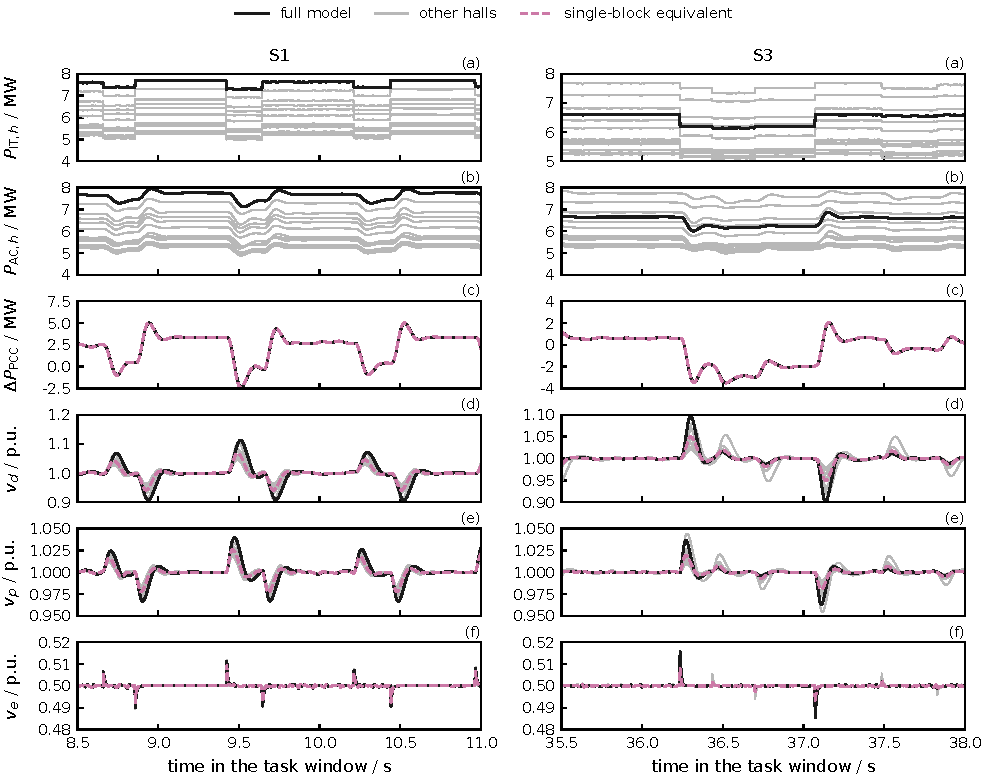
\includegraphics[width=\textwidth]{internal_variables.pdf}
\caption{Internal variables of S1 in the left column and of S3 in the right column, in the realization used in the paper.
(a) Server power $P_{{\rm IT},h}$ and (b) AC input power $P_{{\rm AC},h}$ of every hall.
(c) Change of the PCC active power.
(d) DC-link voltage $v_d$, (e) PSU output voltage $v_p$ and (f) server voltage $v_e$ of every hall.
Black lines show the PCC or the hall with the largest DC-link excursion of the full model in the shown window, which is hall~1 in S1 and hall~2 in S3.
Grey lines show the other halls, and dashed lines the single-block equivalent.}
\label{fig:internal}
\end{figure}

\subsection{Numerical checks}
\label{sec:checks}
The single-block equivalent passes its registered gates at all six operating points.
The equivalent has 179 equations and variables, and the full model has 1873.
Over the six operating points, the largest initial residual is $4.0\cdot10^{-12}$ for the equivalent and $5.8\cdot10^{-12}$ for the full model.
The server power of the equivalent equals that of the full model and of the scenario within $5.8\cdot10^{-12}$~MW, and its static loads equal those of the full model.
A two-second run without input checks that each operating point is an equilibrium.
The largest change of any variable of the equivalent is $5.1\cdot10^{-13}$, and that of the full model is $4.5\cdot10^{-13}$ at the three operating points of the realization used in the paper.
Both models are stable at all six operating points apart from the zero mode of the common rotor angle.
The largest remaining real part of the full model is $-0.117$~s$^{-1}$.
In the positive control of Section~\ref{sec:equivalent}, each eigenvalue of the equivalent is compared with the nearest eigenvalue of the full model.
Their distance is divided by one plus the magnitude of the eigenvalue of the equivalent.
The largest normalized distance is $9.1\cdot10^{-12}$.

The internal-variable reruns reproduce the production runs of both models, with zero difference in the PCC active power and in the DC-link voltage at every output instant.
The four blocks of every hall of the full model agree in every recorded variable within $4.4\cdot10^{-14}$.
The six task-driven runs of the full model keep the converter current below 0.690~p.u., every modulation index below 1.143 times its operating-point value and the DC-link voltage between 0.875 and 1.113~p.u.

\subsection{Evidence limits}
One construction of the single-block equivalent was tested, namely the capacity-weighted average block of Section~\ref{sec:equivalent}.
A single nominal block scaled to the plant rating was not tested.
The comparisons use one electrical design of the 12 halls.
Its parameter ranges are study assumptions and do not form a measured distribution of data-center equipment.

The fast inputs combine literature timing with measured node-power levels.
They are constructed scenarios.
They do not constitute measured PCC transients, measured synchronization across an operating facility or a high-bandwidth measurement of the NLR training cycles.
The polling intervals of the NLR records do not establish the sensor bandwidth.
The phase parameters are the experimental settings of \cite{ko2026oscillations} and not universal workload limits.
Inference remains at a constant request rate within each task window.
The selected job size of 0.125 of the baseline job slots is not a maximum safe job size for a physical facility.

The averaged supply-block model excludes switching ripple, current and modulation limits, protection, battery discharge and bypass switching.
The checks of Section~\ref{sec:checks} therefore describe the response of the model to the selected inputs and do not validate converter protection or field operating limits.
The quasi-static network represents electromagnetic line behavior only through fixed-frequency impedances.
A network with differential electromagnetic states is required to test the resulting approximation across the full 20~Hz band.
The present conclusions concern task-driven PCC quantities and block variables under the stated conditions.

\bibliographystyle{IEEEtran}
\bibliography{references}
\end{document}
